\documentclass[10pt,twocolumn]{article}

\usepackage{amsmath}
% \usepackage{todonotes}
\usepackage{graphicx}
\usepackage{float}
\usepackage{fullpage}
\usepackage{authblk}
\usepackage[%
%    pdftex%
  ,hidelinks%
  ,linktoc=all%               % part of a ToC entry to be made into a link (section/page/all)
  ,unicode%
  ,bookmarksopen=true%
  ,bookmarksopenlevel=0
  ,bookmarksnumbered=true
  %,hypertexnames=false,%     % Correct ToC hyperlinks even with chapter counter reset, but broken biblatex backref.
                              % Instead of using hypertexnames=false, use \renewcommand on \theHchapter,
                              % see http://tex.stackexchange.com/a/6099
  %,draft                     % draft can be used to avoid some strange links errors
]{hyperref}                   % links in pdf document
\usepackage[%
  url=true,%                  % print URLs in references, except for the ones removed below
  backend=biber,%             % use biber instead of bibtex
  firstinits=true,
  sorting=none,
  style=numeric-comp,%          % cite as: (Author 2008)
%   maxbibnames=10,%            % max names in bibliography
%   maxcitenames=2,%            % max names in citation
%   mincitenames=1,%            % if there are more than maxcitenames, shrink to this
  backref=true,%              % prints page numbers (wrong with \frontmatter and hypertexnames=false)
%   dashed=false                % do not replace repeated author with a dash in bibliography
]{biblatex}
\usepackage{nicefrac}
\usepackage[super]{nth}

\usepackage{tikz}
\usetikzlibrary{shapes,arrows,positioning,calc}

\usepackage{siunitx}
\usepackage{todonotes}

\usepackage{mathtools}
\DeclarePairedDelimiter\ceil{\lceil}{\rceil}
\DeclarePairedDelimiter\floor{\lfloor}{\rfloor}

\usepackage{dirtytalk}  % Simple quotation

\usepackage{booktabs}         % better table formatting

\addbibresource{library.bib}  % Bibliography file

\author[*]{F. Rietdijk}
\author[*]{K. Heutschi}
% \author[**]{J. Forss\'{e}n}
\affil[*]{Empa, Swiss Federal Laboratories for Materials Science and Technology, Laboratory for Acoustics/Noise Control, CH-8600 Duebendorf, Switzerland.}
% \affil[**]{Division of Applied Acoustics, Chalmers University of Technology, SE-41296 Gothenburg, Sweden.}

\begin{document}

\title{Auralisation of aircraft with a synthesised emission signal based on features determined from recordings}

\maketitle

\abstract{
Aircraft noise is a major issue in urban areas and is one of the research topics
within the FP7 SONORUS project. Current methods for determining the impact of
aircraft noise on annoyance and sleep disturbance are based on energetic
quantities disregarding the dynamic character of the sound. To obtain a more
complete representation of annoyance, listening tests with audible aircraft
sound promise to determine the impact of the aircraft sound on people more accurately.

A tool was developed to auralise aircraft noise. The propagation model includes,
aside from the typically considered propagation effects like Doppler shift,
atmospheric attenuation and ground reflection, also amplitude and phase
modulations due to atmospheric turbulence. Depending on parameters that are used
to describe the atmospheric turbulence, the amplitude modulations result in
clearly audible modulations and peaks in a spectrogram. Furthermore,
the phase modulations cause additional decorrelation.

An inverse propagation model was developed to compute back from a receiver to
source in time-domain. An automated procedure was developed to extract features
from the resulting signal. These features were then used to directly synthesise
the emission as function of time, and this signal was propagated to the original
receiver resulting in an auralisation that should reproduce the recording
it is based on.

To determine whether the auralisations indeed resembled the recordings, and thus
to validate the auralisation tool, a listening test was conducted. Participants
were presented with recordings and auralisations and had to rate their similarity.
Results indicate that differences exist between the auralisations and recordings.
Improving the synthesis of the blade passing frequency is expected to improve the similarity
between auralisations and recordings.
}

\section{Introduction}

\subsection{Aircraft noise in urban areas}
Due to the rising level of urbanization and the continuing growth of air traffic
the amount of people exposed to aircraft noise increases as well. Aircraft noise
can cause annoyance, sleep disturbance and stress. Annoyance is a biological
process depending on multiple factors that can vary from person to person. If we
consider annoyance due to sound, then certain signal components may be judged
more annoying than others, but this is not reflected in energetic quantities
like $L_{eq}$ or $L_{A,max}$, although in certain cases corrections are applied. To
obtain a better representation of noise we should therefore predict the audible
aircraft sound and study its impact on people \cite{Arntzen2011}.

\subsection{Auralisation}
% Auralisation is a technique to simulate the audible sound of an object or environment.
Auralisation is a method to render audible virtual sound fields \cite{Kleiner1993}.
The method has been used to simulate the audible sound inside
rooms, but also for the sound of
cars \cite{Forssen2009,Maillard2012,Pieren2015,Hoffmann2016,Hoffmann2016a},
trains \cite{Pieren2016},
windturbines \cite{Pieren2014,Heutschi2014},
fans \cite{Merino2016} and
aircraft \cite{Arntzen2014a, Rizzi2016a, Rizzi2016}. Auralisation of outdoor sources
and environments is a key topic of the VASTCON Technical Working Group \cite{Vastcon}.

% Common reasons for generating auralisations is to determine how new and old spaces sound,

Different auralisation methods exist. Often emission synthesis and sound
propagation are separated. This is not always the case because its not always
possible, like e.g. when using a wave-based method
\cite{Hornikx2016,Georgiou2016,Georgiou2016a}.

Common methods for the emission synthesis are spectral modelling synthesis (SMS)
and granular synthesis. Granular synthesis typically uses grains based on
measurements and is a computationally fast method for synthesis. Spectral
modelling synthesis generates a signal through a superposition of two types of
signal components: tones and noise. Whereas with the granular synthesis method
each grain typically corresponds directly to specific conditions, e.g. the speed
of and distance to the source, with spectral modelling synthesis the synthesis
strategy can be considered separate from the underlying model, and therefore a
emission synthesis model can be established that relates tonal and spectral
components to the operational state of the source.

\subsection{Aircraft noise modelling and auralisation}
Aircraft auralisation has been used to study future aircraft types
\cite{Rizzi2013,Rizzi2016,Rizzi2016a} and flight procedures \cite{Sahai2016} but
also to investigate the perceived unpleasantness of aircraft flyover noise as
function of certain temporal parameters \cite{Pate2017}.

Aspects to consider when simulating the sound of aircraft are the different
noise sources on the aircraft, the state of the aircraft and thereby the state
of these sources, as well as the condition of the environment.
% \subsection{Aircraft emission}
The main noise sources of a turbojet aircraft are jet noise, fan and turbine
noise, combustion noise and airframe noise. In the case of turboprop aircraft
the main source is the propellor\cite{Zaporozhets2011}. Fan or propellor noise
is mostly tonal whereas the other sources are broadband noise.
Which exact sources are most relevant depends on the aircraft type and flight
procedure as well as the position of the source with respect to the receiver due
to directivity of the sources \cite{Bertsch2015}.

The aircraft emission prediction tools found in the ANOPP-Source Functional
Module of ANOPP2 \cite{Lopes2016, Tuttle2017} and INSTANT\cite{Sahai2016b}, which is based
on ANOPP, use established models for the noise prediction of the individual
noise sources. The Heidmann model is for example used for fan noise and the
Stone model for jet noise. The Heidmann model in ANOPP models
five sources explicitly, of which three correspond to emission of tones and two
to emission of broadband noise \cite{Arntzen2014a}. The model outputs for each
of these five sources a spectrum in fractional-octaves.
For broadband synthesis in the NAF\cite{Aumann2015}, power of the tonal
components in each band is divided by the amount of tones in that band.
Nowadays the Heidmann model in ANOPP can output the frequencies and amplitudes
of forward and aft radiated fan tones. Only Buzz-Saw noise is still output in
\nicefrac{1}{3}-octaves.

% Both ANOPP2 and INSTANT use spectral modelling
% synthesis to generate an emission signal.

Other models don't describe the contributions from the individual noise
sources or spectral components but merges them together into a total spectrum.
The ECAC Doc29 method \cite{Doc29_fourth_2016} uses the ICAO ANP database and
provides 24 \nicefrac{1}{3}-octave bands, and so does CNOSSOS-EU which has
adopted the \nth{3} edition of Doc29 \cite{Doc29_third_2005}. The Swiss sonAIR
model \cite{Zellmann2016} computes an emission spectrum that is composed of two
source spectra: an engine spectrum and an airframe spectrum. The current Swiss
model, FLULA2, doesn't consider an emission spectrum but instead uses a database
of immission spectra where propagation effects are already included
\cite{EMPA2010,Schaffer2014}.

Aside from ANOPP2 and INSTANT none of the mentioned models make a distinction
between tonal and noise contributions, thereby making them unfit for the use of
aircraft auralisation which requires explicit knowledge about tonal and noise
contributions.

\subsection{Aircraft auralisation tool}
In order to investigate annoyance and sleep disturbance due to aircraft noise
a tool is needed that simulates the audible sound of aircraft in urban
environments. Such a tool would require a) a model to simulate the emission of an
aircraft as function of its operating conditions, b) a sound propagation model,
and c) a sound reproduction setup.

For the development of the sonAIR model \cite{Zellmann2016} sound recordings
were made for a large amount of events nearby Z\"{u}rich Airport
\cite{Zellmann2013}. Along with the sound recordings the position of the
aircraft was registered and for a subset of the events more detailed information
was obtained as well, like e.g. thrust settings. Recordings were made at
multiple positions simultaneously, allowing to determine the directivity of the
noise components.

To study the impact of the current flight procedures and the diverse fleet of
aircraft an auralisation tool is needed that can simulate the audible sound
of each of these aircraft types. Such a tool would require an emission model and
it is investigated whether the sonAIR dataset can be used in conjunction with
spectral modelling synthesis for a generic emission model for aircraft.

Assuming there are no modulations in the aircraft emission the synthesis
strategy would require for each of the tonal components the frequency and power
of the tone as well as the phase relation between the tones. For the broadband
noise components the power as function of frequency would be required. These
features would be needed as function of aircraft state (e.g. thrust settings,
velocity) and as function of source-receiver direction in order to take into
account the directivity.

In addition to a sound propagation model an automated method was
developed to determine these features from the sonAIR dataset
\cite{Rietdijk2015}. The propagation model was used to backpropagate from the
source to the receiver in time-domain, undoing several of the propagation
effects. From the obtained signal the previously described features were
extracted.

% Before continuing the development of an actual emission synthesis model it
% seemed desirable to answer first the following question: can the use of spectral
% modelling synthesis result in plausible auralisations of aircraft?
% Spectral modelling synthesis is commonly used for the synthesis of aircraft
% sound, but the quality of auralisations has not yet been compared to that of the
% determine first whether the chosen synthesis strategy would be a viable method.
A listening test was conducted where participants would
compare recordings to auralisations that were based on the recordings and rate their
similarities. For each auralisation an emission signal is generated with
spectral modelling synthesis that uses as input the features that were
determined with the automated method from a specific recording.

In the following sections we will discuss the different models and methods as
well as the listening test setup in detail. Parameters that are given are those
that were used for the stimuli in the listening test.

% \newpage
\section{Propagation model}

\subsection{Overview}
The propagation model takes into account geometrical spreading, Doppler shift,
atmospheric attenuation and the ground reflection. Furthermore, a model was
developed to include scintillations, that is, fluctuations in the sound due to atmospheric
turbulence \cite{Rietdijk2017}. Convective amplification is supported in the
propagation model but was ignored here.

Figure \ref{fig:propagation_block_diagram} shows
a block diagram of the steps that are taken. Because of source motion all propagation effects are time-variant.
The following sections will describe each of these steps in detail.

\begin{figure}[H]
  \centering
  \resizebox{\columnwidth}{!}{
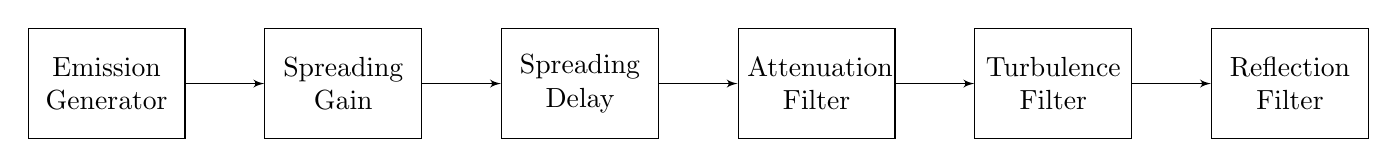
\begin{tikzpicture}[auto, node distance=1cm,>=latex']
\tikzset{
block/.style    = {draw, shape=rectangle, fill=white, minimum height=4em, minimum width=5em, text width=5em, align=center},
}
    % Main nodes
    \node [block]                       (emission)      {Emission\\Generator};
    \node [block, right=of emission]    (spreading)     {Spreading\\Gain};
    \node [block, right=of spreading]   (delay)         {Spreading\\Delay};
    \node [block, right=of delay]       (attenuation)   {Attenuation\\Filter};
    \node [block, right=of attenuation] (turbulence)    {Turbulence\\Filter};
    \node [block, right=of turbulence]  (reflection)    {Reflection\\Filter};

    % Main edges
    \draw [->]  (emission)      --  (spreading);
    \draw [->]  (spreading)     --  (delay);
    \draw [->]  (delay)         --  (attenuation);
    \draw [->]  (attenuation)   --  (turbulence);
    \draw [->]  (turbulence)    --  (reflection);

\end{tikzpicture}}
  \caption{Block diagram of the propagation model. These steps are performed for each propagation path and the resulting signals are summed.}
  \label{fig:propagation_block_diagram}
\end{figure}

\subsection{Geometrical spreading}
Geometrical spreading causes a decrease in amplitude with distance due to divergence and increase
in propagation delay with distance due to the finite speed of sound. Far field
is assumed in which case we obtain the sound pressure at the receiver $p_{\mathrm{rcv}}$
by scaling the magnitude of the sound pressure $p_{\mathrm{src}}$ at some other distance
from the source $r_{\mathrm{src}}$
\begin{equation}
 p_{\mathrm{rcv}} = p_{\mathrm{src}} \frac{r_{\mathrm{src}}}{r_{\mathrm{rcv}}}
\end{equation}

% \subsubsection{Geometrical spreading - phase}
The time-dependent propagation delay, which is relevant for the Doppler shift,
is taken into account by resampling the discretized sound pressure signal with a
Variable Delay Line. Since the signal is discrete and the delay is generally not
an integer multiple of the sample time, an interpolation scheme is required.

Different interpolation schemes exist and in this case a linear interpolation
scheme was chosen due to its simplicity and computational performance \cite{Heutschi2014}.
As a side-effect, linear interpolation causes low-pass filtering of the signal as
well as aliasing. These side-effects can be minimized by choosing another
interpolation scheme, like e.g. Lanczos \cite{Rietdijk2015, Pieren2015}.

% The following describes a method for resampling and linearly interpolating a signal using array processing.
% The actual implementation used a Variable Delay Line (VDL) because a real-time implementation was desired.

For a given sound travel time $\Delta t(t)$ from source to receiver, the index
$k_{e}$ of the signal $s[k_e]$ at the source time-axis is given as
\begin{equation}
 k_{e} = k_r - \Delta t (t) \cdot f_s
\end{equation}
where $f_s$ is the sampling frequency and $k_r$ the sample of the signal at the receiver time-axis. The received signal value $s$ at index $k_e$ is then determined by
\begin{equation}
 s[k_e] = \left( 1 - k_e +  \floor{k_e} \right) \cdot s \left[ \floor{k_e} \right] + \left( k_e - \floor{k_e} \right) * s \left[ \floor{k_e} + 1 \right]
\end{equation}
where $\floor{k_e}$ corresponds to the floor function of $k_e$.
The sound travel time was computed with the following expression for the speed of sound $c = 343.2 \sqrt{ \frac{T}{T_0} }$
where $T$ is the temperature during the event and $T_0 = 293.15$ K the reference temperature.


\subsection{Atmospheric attenuation}
Atmospheric attenuation is accounted for by creating a time-variant filter of length $N_{aa}$
with a magnitude response based on ISO 9613-1:1993\cite{ISO9613-1}. A single-sided magnitude spectrum is calculated as
\begin{equation}
 H_{aa} = 10^{- d \alpha(f) / 20}
\end{equation}
where $d$ is the source-receiver distance in \SI{}{meter} and $\alpha(f)$ the
frequency-dependent attenuation coefficient in \SI{}{\decibel\per\meter}.
% The air pressure, relative humidity, and temperature were recorded during the event.
The impulse response of a magnitude-only filter is non-causal and therefore in
order to create a causal filter a linear-phase filter corresponding to 90
degrees is added. The spectrum is real and even, and therefore the impulse
response is real and even as well. After convolving the signal with the designed
filter the first $N_{aa}/2$ samples were removed to account for the delay caused
by the linear-phase factor.

Convolution was performed using an overlap-save algorithm. The filter length was
4096 samples and the hop size 256 samples. Transitioning to the next impulse
response was done without smoothing.

\subsection{Atmospheric turbulence}
Fluctuations in the atmosphere of wind velocity and temperature affect sound
propagation resulting in fluctuations of both the amplitude and the phase.
Depending on the situation these fluctuations can be clearly audible and
therefore have to be included in order to produce realistic sounding
auralisations.

A method for including phase fluctuations utilizing the mutual
coherence function was presented in \cite{Arntzen2014a, Arntzen2014b, Shin2006}.
The phase fluctuations cause decorrelation between the direct and
ground-reflected contributions resulting in less-pronounced interference
and generally more plausible auralisations.

The authors of this paper developed a model that includes both log-amplitude and phase fluctuations due to
atmospheric turbulence in auralisations \cite{Rietdijk2014, Rietdijk2014a,
Rietdijk2017}. As the aircraft moves through the turbulent atmosphere, the
refractive-index fluctuations are sampled by the waves propagating from source
to receiver. The model considers a line-of-sight situation and assumes a frozen
atmosphere. Other assumptions were a Gaussian applied turbulence spectrum and
spherical wavefront \cite{Wilson1999,Daigle1983}. The model takes into account
saturation of the log-amplitude fluctuations. Details about the model and how it
can be used in auralisations can be found in \cite{Rietdijk2017}.

The autocorrelation function of the Gaussian spectrum is given by \cite{Daigle1983}
\begin{equation}
 C = \frac{\Phi\left(\rho/L\right)}{\rho/L}
\end{equation}
and determines the shape of the log-amplitude $\chi$ and phase fluctuations $S$
spectra. Because of the Wiener-Khinchin theorem we can take the type-1 Discrete
Cosine Transform (DCT-1) to obtain the shape of the autospectra.

The autocorrelation is a function of $\rho$, the spatial separation between two receivers,
perpendicular to the wave propagation direction, and $L$, the correlation
length. Instead of two non-moving receivers we consider a moving source
% that samples the refractive-index fluctuations,
and therefore perform a space-to-time conversion to obtain $C(\tau)$ and $\rho=v_{\bot}\tau$ where
$v_{\bot}$ is the speed of the aircraft perpendicular to the wave propagation
direction.

Gaussian white noise is shaped with this spectrum through a convolution to
obtain log-amplitude and phase fluctuations. Time-variance of the speed is taken
into account not by updating the filter but instead by resampling the sequence of
fluctuations using a Variable Delay Line with a delay based on the time-varying transverse speed.

At this point the fluctuations have a variance of 1. The fluctuations are scaled
by the square root of the desired variances \cite{Daigle1983}
\begin{equation}\label{eq:variances}
 \sigma_{\chi}^2 = \sigma_{S}^2 = \frac{\sqrt{\pi}}{2} \sigma_{\mu}^2 k^2 d L
\end{equation}
which are a function of the variance of the refractive-index fluctuations
$\sigma_{\mu}^2$, wavenumber $k$, source-receiver distance $d$ and correlation
length $L$. This scaling can be time-variant.

The fluctuations are relatively slow, and therefore a filter is constructed to
apply the log-amplitude fluctuations as this also allows to take into account the
frequency-dependency of the fluctuations as shown in equation
\ref{eq:variances}. This filter is obtained by taking the Inverse Discrete
Fourier Transform (IDFT) of $\exp(\chi)$. From equation \ref{eq:variances} it
also follows that the phase-fluctuations have a linear-phase. Therefore, the
phase fluctuations are converted to a propagation delay fluctuation and applied
with a Variable Delay Line.

The variance of the dynamic refractive-index $\sigma_{\mu}^2$ was \SI{3e-5}{}
and the correlation length $L$ \SI{10}{\meter}. The sequences of fluctuations were
initially computed at \SI{100}{\hertz}. The autocorrelation filter had a length
of 8192 samples. The time-variant filter for the amplitude modulations had 512 samples
and hop size was 128 samples. The impulse response transitions were not smoothed.

\subsection{Ground reflection}
While the Image Source Method \cite{Mechel2013} was implemented with image
receivers instead of image sources, we consider here only one additional path,
a ground reflection, and therefore won't go into details about the
implementation of the ISM.

The ground reflection is considered as a second propagation path using a mirror receiver.
% The implementation supports direction-dependent emission signals, but because we had only one emission...
For the ground reflected path the same emission signal was used as for the direct path, thereby ignoring directivity of the sources.
Why the directivity of the source is ignored will become clear in the following sections.

A filter was included to take into account the transfer funtion of the ground. For
the ground reflection the plane wave reflection coefficient was used
\begin{equation}
 R = \frac{Z\cos{\theta}-1}{Z\cos{\theta}+1}
\end{equation}
with impedance $Z$ calculated using Delany and Bazley's 1-parameter model
\begin{equation}
 Z = 1 + 9.08 \left( \frac{1000f}{\sigma}\right)^{-0.75} - 11.9 j \left( \frac{1000f}{\sigma}\right)^{-0.73}
\end{equation}
which is a function of frequency and flow resistivity $\sigma$. The scenarios
considered were landings. Because the area around the airport consists mostly of grass a
flow resistivity of \SI{2e5}{\pascal\second\per\meter\squared} was chosen. The
filter length was 4096 samples and the hop size 256 samples.

% \newpage
\section{Backpropagation and emission synthesis}
% An automated procedure was developed to a) backpropagate from source to receiver
% in time-domain and b) analyze the resulting signal to extract features that could be
% used in the development of an emission model or to directly resynthesise the
% emission.

\subsection{Introduction}
In order to
simulate the audible sound of aircraft an emission signal is needed.
This section describes a method to create an emission signal from features derived from
recordings. An auralisation or pseudo-recording at a receiver position can then
be created by propagating the signal using the propagation model. Figure
\ref{fig:tool:backpropagation:introduction:block-diagram} shows a block diagram
of the steps that are treated in this section.

\begin{figure}[H]
  \centering
  \resizebox{\columnwidth}{!}{
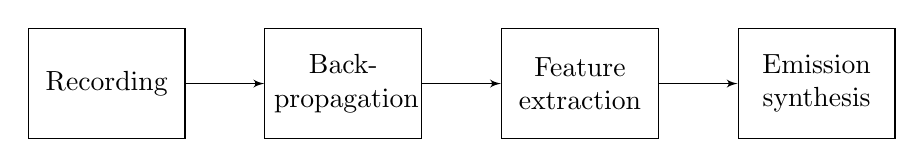
\begin{tikzpicture}[auto, node distance=1cm,>=latex']
\tikzset{
block/.style    = {draw, shape=rectangle, fill=white, minimum height=4em, minimum width=5em, text width=5em, align=center},
}
    % Main nodes
    \node [block]                       (recording)     {Recording};
    \node [block, right=of recording]   (backprop)      {Back-\\propagation};
    \node [block, right=of backprop]    (feature)       {Feature\\extraction};
    \node [block, right=of feature]     (emission)      {Emission\\synthesis};
%     \node [block, right=of emission]    (auralisation)  {Auralisation};

    % Main edges
    \draw [->]  (recording)     --  (backprop);
    \draw [->]  (backprop)      --  (feature);
    \draw [->]  (feature)       --  (emission);
%     \draw [->]  (emission)      --  (immission);

\end{tikzpicture}}
  \caption{Block diagram of the backpropagation, synthesis and auralisation method.}
  \label{fig:tool:backpropagation:introduction:block-diagram}
\end{figure}

\subsection{Measurements for sonAIR}\label{sec:introduction:sonair}
Between 2012 and 2016 a new aircraft noise calculation model called sonAIR was
developed at Empa \cite{Zellmann2013,Zellmann2016}. This semi-empirical model is
based on data obtained from flights that occured at Z\"{u}rich airport in 2013 and
2014.

The main dataset consists of sound recordings at various positions nearby the
airport as well as at larger distances. Sound recordings were made at 44.1 kHz with
microphones at a height of 4 meters above ground level and at several locations
simultaneously. The position of the aircraft were recorded in several ways. Two
special cameras were used to determine the aircraft their position when they
were close to the strip. Radar information was available as well. Furthermore,
for a subset of the events additional data was available from the Flight Data
Recorder (FDR). Some examples of data the FDR provides are the trajectory,
engine shaft rotational frequency and configuration of the gear and flaps. All
data was time-synchronised using GPS receivers. Finally, meteorological data was
available.


For the emission synthesis a signal is generated that is based on some
of these measurements. Figure \ref{fig:figure_trajectory} shows an
overview of the airport, the trajectory and the receiver of the events
considered. Aircraft took off and their height steadily increased from 30 to 260
meters.


\begin{figure}[H]
  \centering
  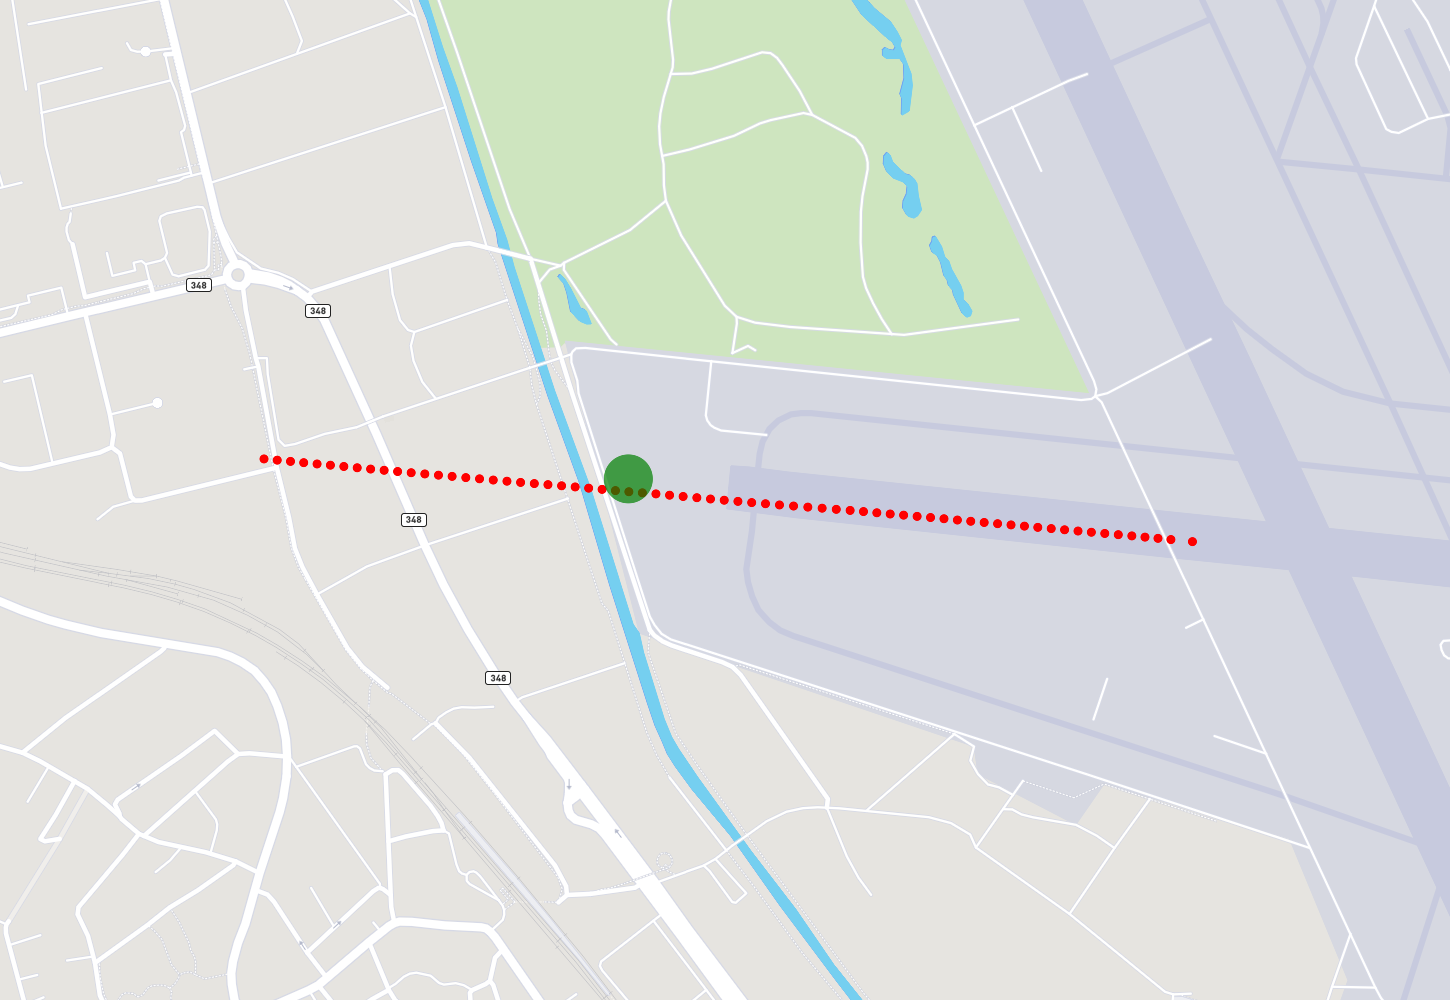
\includegraphics[width=0.3\textwidth]{figures/manual/auralisation-paper/figure_trajectory}
  \caption{Overview of the airport, trajectory and the receiver. The receiver considered
(green dot) is situated slightly north of the trajectory, almost straight underneath the
trajectory.}
  \label{fig:figure_trajectory}
\end{figure}


\subsection{Backpropagation}
An automated procedure was developed to backpropagate from receiver to source in
time-domain. The procedure assumes there is only one propagation path,
the direct path, and that the aircraft can be considered a point source.
As shown in Figure \ref{fig:backpropagation_block_diagram}, the
backpropagation algorithm undoes atmospheric attenuation, the Doppler shift, and
geometrical spreading (magnitude) in that specific order, and using the methods as
described in the previous section.
% A recording is taken, and assuming there were no reflections, the atmospheric attenuation and spherical spreading were undone.
Because only the direct path was considered all parameters that were used in the
backpropagation were based on values corresponding to that path.

\begin{figure}[H]
  \centering
  \resizebox{\columnwidth}{!}{
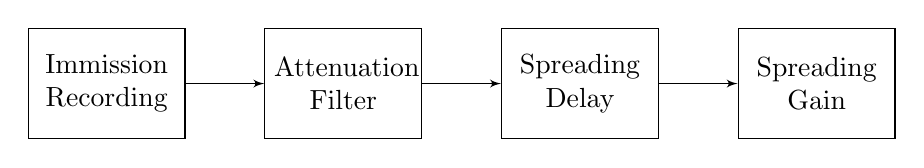
\begin{tikzpicture}[auto, node distance=1cm,>=latex']
\tikzset{
block/.style    = {draw, shape=rectangle, fill=white, minimum height=4em, minimum width=5em, text width=5em, align=center},
}
    % Main nodes
    \node [block]                       (immission)     {Immission\\Recording};
    \node [block, right=of immission]   (attenuation)   {Attenuation\\Filter};
    \node [block, right=of attenuation] (delay)         {Spreading\\Delay};
    \node [block, right=of delay]       (spreading)     {Spreading\\Gain};

    % Main edges
    \draw [->]  (immission)     --  (attenuation);
    \draw [->]  (attenuation)   --  (delay);
    \draw [->]  (delay)         --  (spreading);

\end{tikzpicture}}
  \caption{Block diagram of the backpropagation model. These steps are applied sequentially to a recording in order to obtain a signal in time-domain that corresponds to the emission of the aircraft.}
  \label{fig:backpropagation_block_diagram}
\end{figure}

Application of the backpropagation algorithm results in a time-domain signal
that corresponds to the emission of the aircraft. The emission includes the
effect of convective amplification, i.e., the directivity effects due to source
motion.

The influence of the ground reflection is non-negligible. The backpropagation
model does not undo the ground reflection because it was not expected that this
would result in improved results due to the approximations that would have to be
made. For example, let us assume two clear propagation paths exist. The
immission consists of the contributions from each path. The propagation delays
of each contribution are different. The contributions are therefore
Doppler-shifted differently, and the contributions are generated at different
emission times. Minor differences in emission may exist also due to the
directivity. Furthermore, the reflection coefficient plays a large role and is
only roughly known.

In order to account for the extra contribution, a correction is applied. A soft
ground is still relatively hard and therefore a -3 dB correction was applied to
the power of the features obtained in the next section. Ideally, a microphone on
the ground was used, but the dataset that was available consisted of recordings
at a height of 4 meters.

Figure \ref{fig:recording} shows a spectrogram of a recording. Clearly visible
are the Doppler-shifted tones and the peaks due to atmospheric turbulence. The
most powerful tone corresponds to the blade passing frequency of the fan. The
other tones are Buzz-Saw tones.

Figure \ref{fig:backpropagated} shows a spectrogram of the recording after
backpropagation. The signal after backpropagation is shorter than the recording
due to lack of aircraft position information during the initial propagation
delay. The Doppler-shift has mostly been removed. Aside from small variations,
the tonal components remain constant in frequency over time. The variations are
caused by uncertainties in the measured position of the aircraft and thus the
estimated propagation delay. Artifacts like the mirror-effect and amplitude
modulations due to atmospheric turbulence remain.

\begin{figure}[H]
  \centering
  \includegraphics[width=0.5\textwidth]{figures/generated/recording-to-auralisation/recording}
  \caption{
    Spectrogram of a recording of an A320. }
  \label{fig:recording}
\end{figure}

\begin{figure}[H]
  \centering
  \includegraphics[width=0.5\textwidth]{figures/generated/recording-to-auralisation/reverted}
  \caption{Spectrogram of the recording shown in Figure \ref{fig:recording} after backpropagation to the source.}
  \label{fig:backpropagated}
\end{figure}

\subsection{Feature extraction}\label{sec:tool:emission:features}
Spectral modelling synthesis was chosen as emission synthesis strategy. With
spectral modelling synthesis a signal is generated as a superposition of tones
and bandpass-filtered noise.
Therefore, a method is needed to extract from the backpropagated recordings the
frequency, phase, and level of the tones, as well as the level of the noise as
function of frequency. This section presents a method that was developed for
extracting these features.

The situations considered are take-offs, and therefore the tonal components in
the spectra are not only the blade passing frequency of the fan and its
harmonics, but also \say{Buzz-Saw} tones. The common denominator of the
frequencies of these components is the frequency at which the engine shaft
rotates.

\subsubsection{Motivation for method}
The events considered are short, typically less than 30 seconds, and their
spectra vary considerably over time due to directivity of the source. Thus, in
order to get a sufficiently good directivity resolution, a high temporal
resolution is needed, and that limits the possibility to average over time. The
frequency resolution, however, also matters. The emission may contain Buzz-Saw
harmonics with a fundamental frequency below 100 Hz. While that gives some
freedom for using a lower frequency resolution, first the actual tonal
components need to be detected and thus distinguished from the broadband noise.

While already corrected for in the backpropagation, the Doppler shift may make
it difficult connecting obtained frequency-components at one step to those
obtained the step later. Therefore, frequency-tracking algorithms were
considered \cite{Lampert2010}, notably Hidden Markov Models. Due to their
complexity such solutions were not pursued further.

Tone-detection in the frequency-domain is in its simplest form a matter of peak
detection for which a range of algorithms is known. However, a robust algorithm
is needed that can distinguish between the tonal components and broadband noise
peaks.

Initially, the complex cepstrum\footnote{The complex cepstrum is defined as
$c[n] = F^{-1}\left\{\log_{10}{\left( F \left\{x[n]\right\} \right)}\right\}$.}
was used to determine the fundamental frequency of the Buzz-Saw harmonics.
The method was reliable for determining the
fundamental frequency. Because all the tonal components considered are multiples
of this fundamental frequency, all their frequencies would then be known as
well. Unfortunately, the frequency-resolution, or more precisely the
quefrency-resolution, was not high enough to reliably predict the frequency of
the high-frequent components.

\subsubsection{Tone-seeking algorithm}
Annex C of ISO 1996-2:2007 \cite{ISO1996-2_2007} describes an objective method
for assessing the audibility of tones in noise and a significant part of the
method describes a tone-seeking algorithm. The tone-seeking algorithm works in
frequency-domain on a narrowband power spectrum. An estimate of the narrowband
spectrum is obtained using Welch's method. The time signal is split in chunks, a
Hanning window is applied to each chunk, and a modified periodogram is determined for
each chunk. Finally, linear averaging over the chunks results in Welch's
estimate of the power spectral density.

In frequency-domain, the tone-seeking algorithm first determines noise pauses,
which are local maxima with a probability of a tone. Noise pauses span multiple
frequency lines, and their starts and ends can be found when the difference
between two adjacent lines is larger than $\Delta$ dB, where $\Delta$ is the
tone-seeking criterion. The next step is to assess whether tones exist in these
noise pauses. Each frequency bin or line is assigned a label indicating whether
it is part of a tone or whether it is masking noise.

The power of the lines that are part of a tone are integrated. A correction is
made for the masking noise contributions to those lines by estimating their
contribution from a regression through the lines marked as noise within a
portion of the critical band\footnote{A critical band is the bandwidth of a
filter created by the cochlea, the auditory part of the inner ear.} around the
centerfrequency of the tone. Furthermore, a 1.8 dB correction is applied as
correction for the Hanning window.

\subsubsection{Extension and modifications}
The tone-seeking algorithm is capable of detecting many of the tonal components
but not all of them. Therefore, the algorithm is modified and extended.
Because the tones of interest are all multiples of a
fundamental frequency, the goal is to determine this fundamental frequency
sufficiently accurate. The assumption was therefore made that all tones found by the
tone-seeking algorithm from the standard were harmonics and that the fundamental
frequency was within a specified range.
The fundamental frequency is then given
\begin{equation}
 f_{0} = \mathrm{gcd}\left(f_1, f_2, \dots, f_n \right)
\end{equation}
where $\mathrm{gcd}$ is the \emph{greatest common divisor}.
Implementations of the $\mathrm{gcd}$ operator attempt to find an exact solution.
Due to errors in the estimation of the frequency of the tones and because some tones are
not harmonics, an exact solution does not exist. Given an initial estimate of
the fundamental frequency, one could define an error as the sum of the squared
deviation between the target order of the harmonics and the actual estimated
order
\begin{equation}\label{eq:tool:features:error}
 e = \sum_{i=0}^{n} \left( \frac{f_i}{f_0} - \mathrm{round}\left(\frac{f_i}{f_0}\right) \right)^2
\end{equation}
An estimate of the fundamental frequency is obtained by minimising this error.

According to the standard an A-weighted signal should be used. Because the
frequencies of the tonal components are of interest, and not their audibilities,
an unweighted signal is considered instead. Because at the start and the end of
the signal the signal-to-noise is relatively low, the backpropagation algorithm
may cause unwanted amplification of the background noise. Therefore, the signal
was low-pass filtered with a \nth{4} order Butterworth low-pass filter with a
cut-off frequency at 10 kHz. Furthermore, in order to obtain an accurate
estimation an averaging-time of one minute is required, however, this could not
be done as explained. Instead, two-second windows without overlap were used, and
these windows were divided into 10 chunks in order to estimate a power spectrum
with a resolution of about 5 Hz. A two-second window proved to be a good balance
between temporal resolution and frequency resolution.

The tone-seeking algorithm is first ran with a tone-seeking criterion of 1 dB to
detect tonal components and obtain their centerfrequencies. A fundamental
frequency estimation is then done by minimising the error in equation
\eqref{eq:tool:features:error}. The next step is to determine the power of all
harmonics. That was done by explicitly setting noise pauses for each of the
harmonics, forcing the tone-seeking algorithm to determine tones.
The noise-pause bandwidth was set to a value that was a function of the fundamental
frequency $f_0$ in order to automatically scale. Because adjacent noise pauses
should not overlap the bandwidth should be smaller than $f_0$. The noise pause
bandwidth was set to $0.2 f_0$ as this value appeared to work well for
estimating the power of the \say{Buzz-Saw} harmonics. The level of the tones are
then estimated as described by the standard.

The broadband noise or \say{masking noise} was integrated in
\nicefrac{1}{6}-octaves and a Hanning-window correction of 1.8 dB was applied.
The -3dB bandwidth of the tones was recorded as well, although these values may
be inaccurate due to the 5 Hz frequency-resolution. The bandwidth of the tonal
components depends on various aspects, like frequency or phase modulations at
the source or during propagation, e.g. due to atmospheric turbulence. The direct
and reflected contribution are Doppler-shifted slightly differently and that
causes either double peaks or a single broader peak. But also averaging time and
window shape play a role.

\subsection{Emission and immission synthesis}\label{sec:tool:synthesis:synthesis}
% As mentioned before the emission was synthesised using spectral modelling
% synthesis.
With the extracted features, which were obtained as function of time and at
several receiver positions, it is possible to develop an emission model that
takes into account directivity of the spectral components. Such emission model
would then output input for the SMS synthesiser, and the created emission signal
would be propagated to a receiver location.

An important question to ask is whether the described methodology of extracting
features, synthesising an emission signal and propagating it would result in
plausible auralisations. For example, it could be possible that the chosen
synthesis strategy and features cannot reproduce certain characteristics in the
sound. Therefore, the next chapter describes a comparison between auralisations
and recordings with the auralisations based on recordings.

For a specific event and receiver, the immission was backpropagated and features
were extracted. These features were used to re-synthesise the emission. The
emission signal was propagated to the receiver, and a direct path and a single
reflection were considered. The assumption was made that the emission is
identical for the emission angles corresponding to direct and reflected path.

The feature extraction method provided frequencies and levels of tonal
components as function of time. Variations in the frequencies as function of
time could be observed, but with a two second window that would result in only
few data points. Variations in frequency were therefore ignored and computed was an
average value for the fundamental and each of the harmonics.

As mentioned in the previous section, values for the phase of the tones could
not be obtained, and therefore values had to be chosen. Because the harmonics
are \say{Buzz-Saw} noise, a phase corresponding to a sawtooth signal was
initially assumed. Participants in a preliminary test found the simulations
sound metallic compared to the recordings.
Therefore, the assumption was made that the initial phase relation between the
Buzz-Saw tones was entirely lost and could therefore be chosen randomly, in
which case the probability distribution would likely be uniform as otherwise a
certain initial phase would still be preferred.

Figure \ref{fig:synthesis} shows a spectrogram of the emission synthesis. The
level of the tonal components and the broadband noise varies over time. The
blade passing frequency is not clearly visible. The feature extraction algorithm
underestimated the levels of the blade passing frequency and its harmonics. As
explained in \ref{sec:tool:emission:features} tones were searched for in noise
pauses. These noise pauses were \say{created} after the fundamental frequency
was determined. The bandwidth of these noise pauses was relatively small because
they were tuned for the \say{Buzz-Saw} tones. An improvement would be to look in
a larger noise pause bandwidth or bandwidth for these tonal components, however,
that requires explicit knowledges of the amount of blades.

Figure \ref{fig:auralisation} shows a spectrogram
of the auralisation at the receiver. The Doppler-shifted tones and the
mirror-effect are clearly visible. The Doppler-shifted tones are not very
smooth. This is due to fluctuations in the measured aircraft position and a smoothing filter
could reduce impact of these uncertainties.

% \newpage
% \afterpage{
\begin{figure}[H]
  \centering
  \includegraphics[width=0.5\textwidth]{figures/generated/recording-to-auralisation/synthesis}
  \caption{Emission synthesis of the aircraft. Inputs to the emission synthesiser were obtained by applying the feature-extraction algorithm to the signal shown in Figure \ref{fig:backpropagated}.}
  \label{fig:synthesis}
\end{figure}


\begin{figure}[H]
  \centering
  \includegraphics[width=0.5\textwidth]{figures/generated/recording-to-auralisation/auralisation}
  \caption{Auralisation of the event shown in Figure \ref{fig:recording} .
  }
  \label{fig:auralisation}
\end{figure}
% }


\section{Subjective validation of auralisations}

\subsection{Listening test}
A listening test was done to check the plausiblity or perceptual validity of the
auralisations and a comparison was therefore made between recordings and
auralisations.
The hypothesis is that \emph{recordings and auralisations of aircraft of the same
type and under similar conditions are samples of the same group}.
Audible differences are likely to occur and are also acceptable, because even
among recordings of the same aircraft type there are audible differences.

Psychoacoustic measures were not measured. Instead, an overall similarity
between stimuli was determined by letting participants rate how similar they
found two sounds to be, where similar is defined as entities that are alike or
have characteristics in common.

Recordings were compared not only with auralisations,
but also with other recordings, and similarly, auralisations with other
auralisations. Each of these comparisons can be considered a group. If the
hypothesis is valid, then the distribution of the group with comparisons between
recordings and auralisations, should be the same as the other two distributions.

\section{Method}

The goal of the listening test was to determine whether the auralisations sound
similar to the recordings they were based on. Participants were presented with
pairs of stimuli and asked to rate how similar they sounded, overall.

Eight different sounds were considered and they were each 12 seconds long. The
sounds include the approach of an aircraft, its fly-over and its distancing.
Because the character of the sounds varies considerably over time, they were
each split into parts of four seconds, corresponding to the approach, fly-over
and distancing. The listening test was also divided in these three parts. First,
participants were presented to all approach stimuli, then all fly-over stimuli
and finally all distancing stimuli. In each test part all stimuli combinations
were considered. Therefore, each part consisted of 28 pairs of stimuli of four
seconds.

Of the eight sounds four were recordings, and four were auralisations.
The recordings were randomly chosen from the sonAIR dataset. Each
auralisation was based on one of the recordings. Two aircraft types were
considered, an A320 and a RJ1H, as well as two events per aircraft type.
Fade in and fade out was applied to the stimuli. The signals were mono and
presented with headphones. Head-related transfer functions were not included.

Similarity is relative, and therefore an anchor is typically used. For each
part, participants were first given the set of stimuli, in order to become
familiar with the type of sounds and the spread in the sounds of that part, and
then continued with rating the pairs. The rating was done on an eleven point
Likert scale. The left side of the scale said ``not so much'' and the right side
``very much''. The scale was not numbered. The order of the stimuli was
randomised for each test and each part.

Figures \ref{fig:listening:results:recording-A320} and
\ref{fig:listening:results:simulation-A320} show spectrograms of some of the
stimuli that were used. The blade passing frequency and harmonics are not as
prominent in the auralisation as they are in the recording. The approach-part of
the auralisation spectrogram shows a part where the signal was zero and this is
due to the initial propagation delay. This was supposedly accounted for by
creating longer auralisations and then selecting the part where there was
signal, but judging from the spectrogram and inspection of the audio files, an
error was made. This was noticed only after the listening tests. The errors are
0.15 and 0.35 seconds in the case of the RJ1H samples, and 0.65 and 0.75 seconds
in case of the A320 samples.


% \newpage
% \afterpage{
\begin{figure}[H]
  \centering
  \includegraphics[width=0.5\textwidth]{figures/generated/listening/recording-A320}
  \caption{Spectrograms of the approach, fly-over and distancing parts of a recording of an A320.}
  \label{fig:listening:results:recording-A320}
% \end{figure}
%
% \begin{figure}
  \centering
  \includegraphics[width=0.5\textwidth]{figures/generated/listening/turbulence-A320}
  \caption{Spectrograms of the approach, fly-over and distancing parts of an auralisation of an A320.}
  \label{fig:listening:results:simulation-A320}
\end{figure}
% }
% \clearpage

% \newpage
\section{Results}
The results of the participants were scaled linearly from 0 to 1 with 0
corresponding to ``not so much'' and 1 corresponding to ``very much''.
% Not all of the participants used the entire scale, and therefore they were rescaled per
% participant and per test part to use the full scale.
There were 17 participants, all graduate students, and of which the majority
studied acoustics. The results that are shown are obtained after joining the
data of all participants. % and all three test parts.
% Update raw results??
The listening test data can be found at \cite{Rietdijk2017a} and the
raw results along with a brief analysis at \cite{Rietdijk2017b}.

Table \ref{table:listening:results:analysis-parts} shows the sample mean $\mu$,
sample standard deviation $\sigma$ and amount of samples $n$ per group. Averaging was
done over participants. Table
\ref{table:listening:results:analysis-with-approach} is similar, with averaging
done over the three test parts as well. Table
\ref{table:listening:results:analysis} is like Table
\ref{table:listening:results:analysis-with-approach}, however, with all approach
parts excluded. Because participants are a sample of the actual
population, $n-1$ degrees of freedom were considerd for the computation of the
standard deviation and the standard error of the mean $\sigma/\sqrt{n}$.

The following figures show per group a normalised histogram and a kernel density estimation\footnote{ A kernel density estimation can be seen as a continuous version
of a histogram. Each sample is replaced by a kernel function centered at the
value of the sample. The curves are then summed to obtain a density and finally
normalised so that the area under the resulting curve is 1. }. A Gaussian kernel
was used.
% Figure \ref{fig:listening:ratings-kde-overall} shows the distribution of the
% similarity ratings grouped by aircraft and stimuli type combinations. The
% vertical axes show kernel density estimations of how common the given ratings
% were
In Figure \ref{fig:listening:ratings-histograms-all} averaging is done over all participants and all parts.
In Figure \ref{fig:listening:ratings-histograms-no-approach} averaging is done over all participants, as well as the the fly-over and distancing parts.
Figures \ref{fig:listening:ratings-histograms-approach}, \ref{fig:listening:ratings-histograms-flyover} and \ref{fig:listening:ratings-histograms-distancing}
consider the approach, fly-over and distancing separately. In these figures averaging is done only over participants.

Participants mentioned they noted larger differences at especially the approach of the events and the distancing.
A common answer to the question how many different aircraft they heard was ``two or three``.
Occasionally, the answer would start at ``two`` but go to ``two or more`` after they
were told they were listening to not only recordings but also simulations. Some
participants were surprised when told that simulations were included,
others said they had thought so, and a few of the participants were already
aware the test was possibly going to contain simulations.

% \newpage
\begin{table}[H]
  \centering
  \caption{The mean value $\mu$, standard deviation $\sigma$ and amount of samples $n$ per aircraft type combination, and stimuli type combination. Averaging was done over participants and parts.}
  \label{table:listening:results:analysis-with-approach}
  \input{figures/generated/listening-analysis/table_analysis.tex}
\end{table}

\begin{table}[H]
  \centering
  \caption{The mean value $\mu$, standard deviation $\sigma$ and amount of samples $n$ per aircraft type combination, and stimuli type combination. Averaging was done over participants and parts, \emph{excluding the approach parts}.}
  \label{table:listening:results:analysis}
  \input{figures/generated/listening-analysis/table_analysis_no_approach.tex}
\end{table}

% \newpage

\begin{table}[H]
  \centering
  \caption{The mean value $\mu$, standard deviation $\sigma$ and amount of samples $n$ per test part, aircraft type combination, and stimuli type combination. Averaging was done over participants.}
  \label{table:listening:results:analysis-parts}
  \resizebox{\columnwidth}{!}{
  \input{figures/generated/listening-analysis/table_analysis_parts.tex}
  }
\end{table}

\begin{figure}[H]
  \centering
  \includegraphics[width=0.5\textwidth]{{{figures/generated/listening-analysis/histograms}}}
  \caption{Normalised histogram and kernel density estimate per group. Averaging was done over all participants, and all parts.}
  \label{fig:listening:ratings-histograms-all}
\end{figure}

\begin{figure}[H]
  \centering
  \includegraphics[width=0.5\textwidth]{{{figures/generated/listening-analysis/histograms_no_approach}}}
  \caption{Normalised histogram and kernel density estimate per group. Averaging was done over all participants, and the fly-over and distancing parts.}
  \label{fig:listening:ratings-histograms-no-approach}
\end{figure}

% \begin{figure}[H]
%   \centering
%   \includegraphics{{{figures/generated/listening-analysis/histograms_approach}}}
%   \caption{Normalised histogram and kernel density estimate per group for the approach part. Averaging was done over all participants.}
%   \label{fig:listening:ratings-histograms-approach}
% \end{figure}
%
% \begin{figure}[H]
%   \centering
%   \includegraphics{{{figures/generated/listening-analysis/histograms_flyover}}}
%   \caption{Normalised histogram and kernel density estimate per group for the fly-over part. Averaging was done over all participants.}
%   \label{fig:listening:ratings-histograms-flyover}
% \end{figure}
%
% \begin{figure}[H]
%   \centering
%   \includegraphics{{{figures/generated/listening-analysis/histograms_distancing}}}
%   \caption{Normalised histogram and kernel density estimate per group for the distancing part. Averaging was done over all participants.}
%   \label{fig:listening:ratings-histograms-distancing}
% \end{figure}

% \newpage
\section{Discussion}
Consider tables \ref{table:listening:results:analysis-with-approach} and
\ref{table:listening:results:analysis}. In both tables the sample
standard deviations are around 0.25. The spread in the mean within the tables is
large, but the difference in mean values between the two tables is small. While
the largest difference is 0.05, which is about two standard errors, for the
majority of groups the difference is about one standard error.

Table \ref{table:listening:results:analysis-parts} does not average over the
three parts. Again, the standard deviation of the groups is mostly around 0.25,
although a notable exception is the group in which two recordings of A320's were
compared. The standard deviation is only 0.09 and the mean 0.89. Comparing that
with the other groups, implies the two recordings this group consists of are
relatively closer to each other than those in other groups. The standard
deviation of the approach groups with the faulty auralisations is similar as
that of the other groups.

The highest mean values are achieved when comparing similar aircraft types,
regardless of whether the stimuli were recordings or auralisations. However,
when comparing a recording with an auralisation the mean value is lower. The
mean values of the groups comparing recordings and auralisations are
systematically below those of the groups comparing recordings or auralisations.
That would imply the hypothesis that \say{recordings and auralisations of aircraft of the same
type and under similar conditions are samples of the same group} is not true.

Figures \ref{fig:listening:ratings-histograms-all} and
\ref{fig:listening:ratings-histograms-no-approach} show normalised histograms
and kernel density estimates. The difference beween the two figures is that the
latter does not include approach samples. No notable differences can be observed
in the figures, implying the approach samples are \say{average}.


The similarity rating is a value given by participants after performing a
comparison of two items, and comparing them on whichever aspects they choose to
consider. Therefore, it is likely that the distributions are Gaussian. However,
the ratings could only be given on a limited range and that may skew the
distributions. In most cases the distributions do not appear to follow a Gaussian curve.

The recordings of the A320's (top-left) are judged to be very similar to each other, and
the recordings of the RJ1H's (bottom-left) as quite similar to each other as well although
slightly less. The A320's are not rated as very similar to the RJ1H's (center-left) and
therefore it appears that the participants can discriminate between the two
aircraft types.
For the auralisations, the results are similar in case of the A320's (top-right)
and the RJ1H's (bottom-right), although less convincing. Furthermore, in this case the
dissimilarity between the A320's and the RJ1H's isn't as large (center-right). In fact, this
distribution is relatively closer to the other two distributions than is the
case with the recordings, implying the auralisations, regardless of aircraft
type, all sound more alike. That is, they all sound more like another aircraft type.

Were the hypothesis valid, then the curves in the top would have to overlap, and
the curves in the bottom as well. While the distributions of the groups that
compare auralisations are quite similar to the distributions comparing
recordings, they are not similar to the groups comparing auralisations with
recordings. That would again imply the hypothesis is not true and that the
auralisations may appear to be different types of aircraft.

% % The groups ``(rec, sim)'' contain pairs consisting of a recording and an auralisation, and the similarity ratings of these two groups are similar to the ``(A320, RJ1H)''
% % groups in Figure \ref{fig:listening:ratings-aircraft-type-combinations}. Therefore,
% % it would appear that listeners can discriminate between aircraft types, but that
% % the auralisations are considered to be of different aircraft types than the
% % recordings they are based on.

While not shown, similar curves were created per test part.
Aside from the A320 distancing recordings that were mentioned before,
there do not appear to be significant differences between the parts.
In case of the RJ1H the distancing stimuli seem to be relatively close to each other.

The participants mentioned relatively larger differences in the stimuli that
correspond to the approach of the aircraft (approach stimuli). During the
approach the tonal components are clearly audible compared to other parts of the
events due to the directivity. The feature-extraction algorithm was known to
underestimate the power and bandwidth of the blade passing frequency and its
harmonics because the algorithm was tuned for the Buzz-Saw tones. Therefore, a
likely explanation is that this underestimation of power and bandwidth is
causing audible differences between recordings and auralisations.
Another cause could be the initial delay error.

The author noticed after the listening test that the initial phase of the tones
was Gaussian distributed instead of uniform (see section
\ref{sec:tool:synthesis:synthesis}) resulting in a most probable zero degrees
initial phase for all tonal components. That may affect how the sound is
perceived.

The listening test considered only two events per aircraft type. In order to
correctly represent the spread that exists in recordings of a certain group, in
this case, an aircraft type. Future tests should therefore consider more events
and investigate the spread that already exists in the similarity between
recordings. Increasing the test size would, however, significantly increase the
test size, which is the reason only two events per aircraft type were
considered.


\section{Conclusion}
Aircraft noise has a negative impact on humans. To further study its impact on
humans a tool was developed to simulate the audible sound caused by
fly-overs of airplanes. The goal was to develop a tool that can create
auralisations of the current fleet of aircraft that sound plausible.

The auralisation tool consists of an emission synthesiser and a propagation
model based on geometrical acoustics. The emission synthesiser used spectral
modelling synthesis as synthesis strategy and used features extracted from
recordings as input. These features were automatically extracted from a signal
that was obtained after applying an inverse propagation model to a recording.
To verify whether the auralisations sound similar to recordings of the
respective airplane types, a listening test was conducted.

In a listening test participants were presented with two stimuli
at a time and were asked to rate on a categorical scale the similarity of the two stimuli,
where the two stimuli could be recordings, auralisations, or one of each. The
hypothesis was that \emph{recordings and auralisations of aircraft of the same
type and under similar conditions are samples of the same group}. This
hypothesis would be true, if the distribution of the group with comparisons
between recordings and auralisations would be the same as the other two
distributions.

There were clear differences in the distributions, implying the hypothesis is
not true. In case of the recordings, the participants were clearly discriminating
between the two different aircraft types that were considered. With the
auralisations this was not as clear, however, and it would appear that the
auralisations sound more as different aircraft types.

An incorrect reproduction of the blade passing frequency and its harmonics is
the likely cause of the dissimilatity between the auralisations and recordings.
The feature-extraction algorithm was tuned for the relatively small bandwidth of
the Buzz-Saw tones and is therefore underestimating the power and bandwidth of
the blade-passing frequency and harmonics.

Therefore, future work should emphasise on further improving the simulations.
The authors think that the most important point to improve is the simulation of
the blade passing frequency and harmonics, and that would require a better
estimation of their powers and bandwidths. Aside from that, it would seem the
auralisation tool is capable of delivering plausible auralisations.

\section{Acknowledgement}
The research leading to these results has received funding from
the People Programme (Marie Curie Actions) of the European Union's Seventh
Framework Programme FP7/2007-2013 under REA grant agreement number 290110,
SONORUS "Urban Sound Planner".
% }

\printbibliography[heading=bibintoc]

\end{document}

